% !TeX root = ../Main/XMU.tex
\chapter{实验结果和讨论}{Result and Discussions}
\section{实验细节}{Implementation Details}
\label{sec:implementation}
深度学习网络的训练环境和测试环境如下:
\begin{itemize}
	\item{操作系统:}Ubuntu 16.04
	\item{CPU:}Inter i7 7800k
	\item{GPU:}Nvidia Geforce TitanXP
	\item{内存:}16G
\end{itemize}
实验所需的材料(包括代码、训练集、测试集)发布在github上\footnote{link: https://github.com/uhomelee/DeepInverseKinematicsSolver}。整个训练过程需要大约36小时。
\begin{figure}[!htbp]
	\centering
	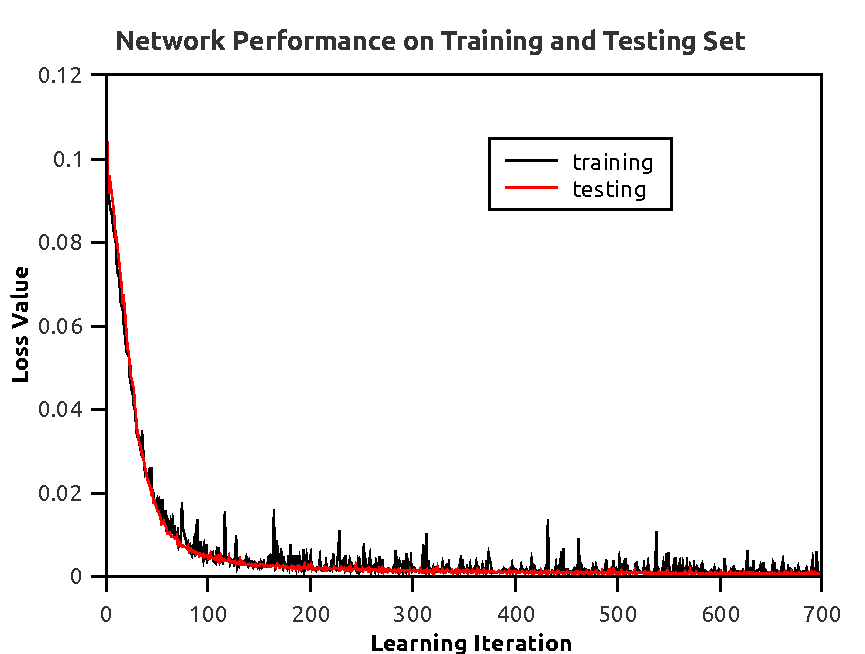
\includegraphics[width=0.75\linewidth]{loss_train_test}
	\caption[]{\label{fig:train_test}
		训练集和测试集比较
	}
\end{figure}
\begin{figure}
\centering
\subfigure[篮球运球动作] {
\label{fig:train_screenshot_dribble}
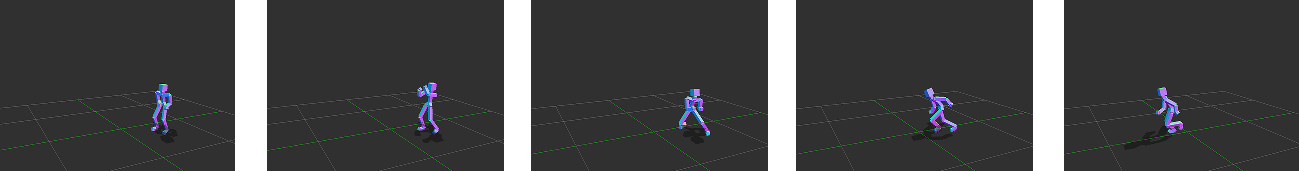
\includegraphics[width=\textwidth]{train_screenshot_dribble}
}
\subfigure[篮球投篮动作] {
\label{fig:train_screenshot_shooting}
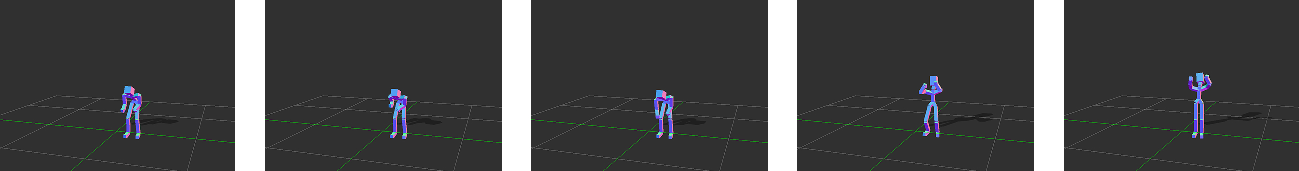
\includegraphics[width=\textwidth]{train_screenshot_shooting}
}
\subfigure[芭蕾舞动作] {
\label{fig:train_screenshot_dancing}
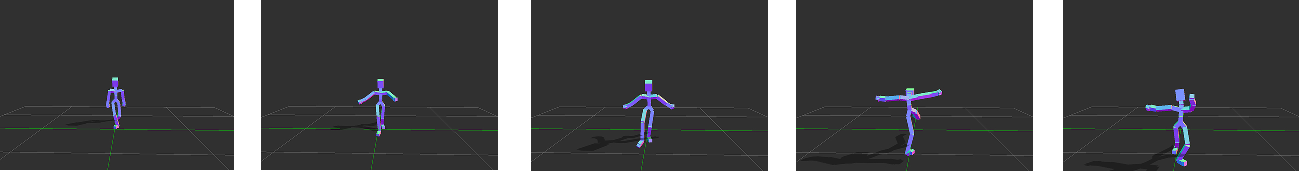
\includegraphics[width=\textwidth]{train_screenshot_dancing}
}
\caption{训练动作数据库合成动作}
\label{fig:train_screenshot}
\end{figure}
\begin{figure}
\centering
\subfigure[坐-起立动作] {
\label{fig:test_screenshot_gettingup}
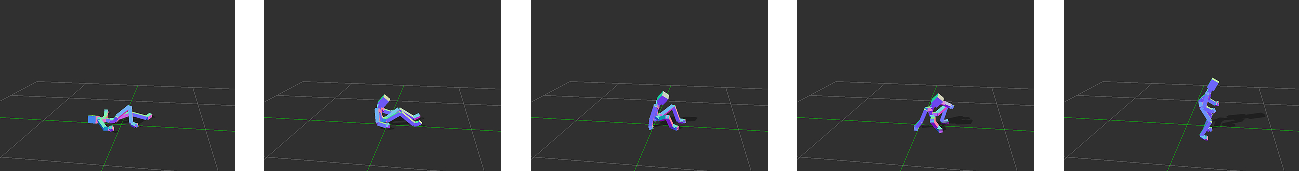
\includegraphics[width=\textwidth]{test_screenshot_gettingup}
}
\subfigure[篮球运球动作] {
\label{fig:test_screenshot_dribbling}
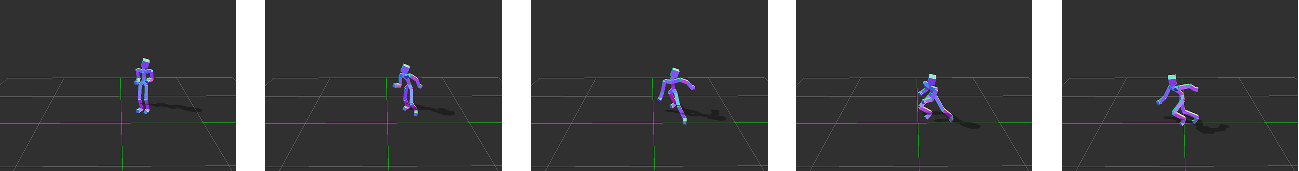
\includegraphics[width=\textwidth]{test_screenshot_dribbling}
}
\subfigure[翻跟头动作] {
\label{fig:test_screenshot_rolling}
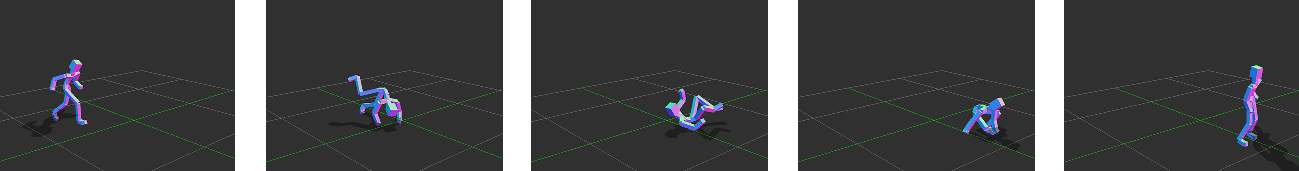
\includegraphics[width=\textwidth]{test_screenshot_rolling}
}
\caption{测试动作数据库合成动作}
\label{fig:test_screenshot}
\end{figure}
\section{实验结果}{Result}
\subsection{训练集和测试集结果}{Results on Training and Testing Dataset}
神经网络的训练集和测试集输出结果全部通过MATLAB脚本替代原有的BVH文件的数据值,并通过BVH PLAYER进行播放。训练结果可以通过两方面来检测,一是BVH文件的播放后的视觉效果,二是观察训练过程中训练集和测试集的损失函数值。


% \cref{fig:train_screenshot}展示了来自训练集的合成动作(包括篮球运球、投篮和芭蕾舞动作)。这些示例都需要角色对象进行精细的操作(例如对篮球的掌控)以及与环境频繁的交互(例如地面上的脚部支撑)。 这些动作的求解都需要ik解算器具备较高的精度。 一般来说,训练样本的最优的平均损失$<10^{-5}$,实际的预测的欧拉角和真实值的相差约在$\pm0.01^{\circe}$之间。

\cref{fig:test_screenshot}展示了来自测试集中的合成动作(包括从地面起立、篮球运球和翻跟斗)。
尽管这些例子中的动作并未包含在训练集中,但IK解算器仍可以解决该问题并产生符合自然姿态的动作。需要指出的是,测试集上的结果并未出现过拟合的情况,如\cref{fig:train_test}所示,训练集和测试集的损失函数值随着迭代次数的递增而下降,最终的结果测试样本的平均损失在$10^{-4}~10^{-5}$之间。通过实验,在全连接(FCN)模型中,虽然训练集上的网络性能表现良好,但在测试集上非常容易出现过拟合的情况。

\begin{figure}[!htbp]
	\centering
	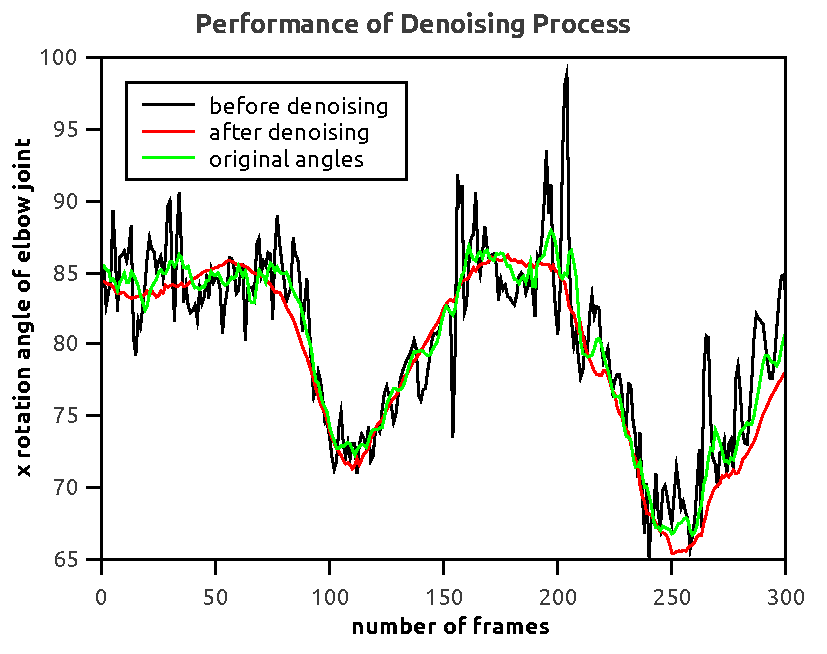
\includegraphics[width=0.75\linewidth]{denoising}
	\caption[]{\label{fig:denoising}
		去噪滤波器处理前后和真实值对比
	}
\end{figure}
\subsection{去噪滤波器结果}{Result on Denoising Filter}
尽管网络模型的损失函数在训练结束后收敛得非常小,但\textbf{IK}问题的求解的另一个需要考虑的因素是合成连贯动作后的自然度。考虑到$\mathbf{PE}$组件的输出在BVH PLAYER上播放时在某些复杂的动作(例如频繁的上下抬手、大范围的移动等情况)时出现的视觉上的抖动问题,对$\mathbf{PE}$组件的输出进行了降噪,具体的方法见\ref{sec:denoising}。如\cref{fig:denoising}所示,降噪的结果可以说是非常显著的。在BVH PLAYER上播放后,原先已经符合视觉上自然流畅的动作会显得更加自然(避免了太大角度的弯曲,违背了人体关节的旋转极限);原先有抖动的文件,在经过降噪后,基本可以做到流畅和自然。
\label{res:denoising}

\subsection{姿态估计结果}{Result on Posture Estimation}
\begin{figure}
\centering
\subfigure[] {
\label{fig:2dtobvh1}
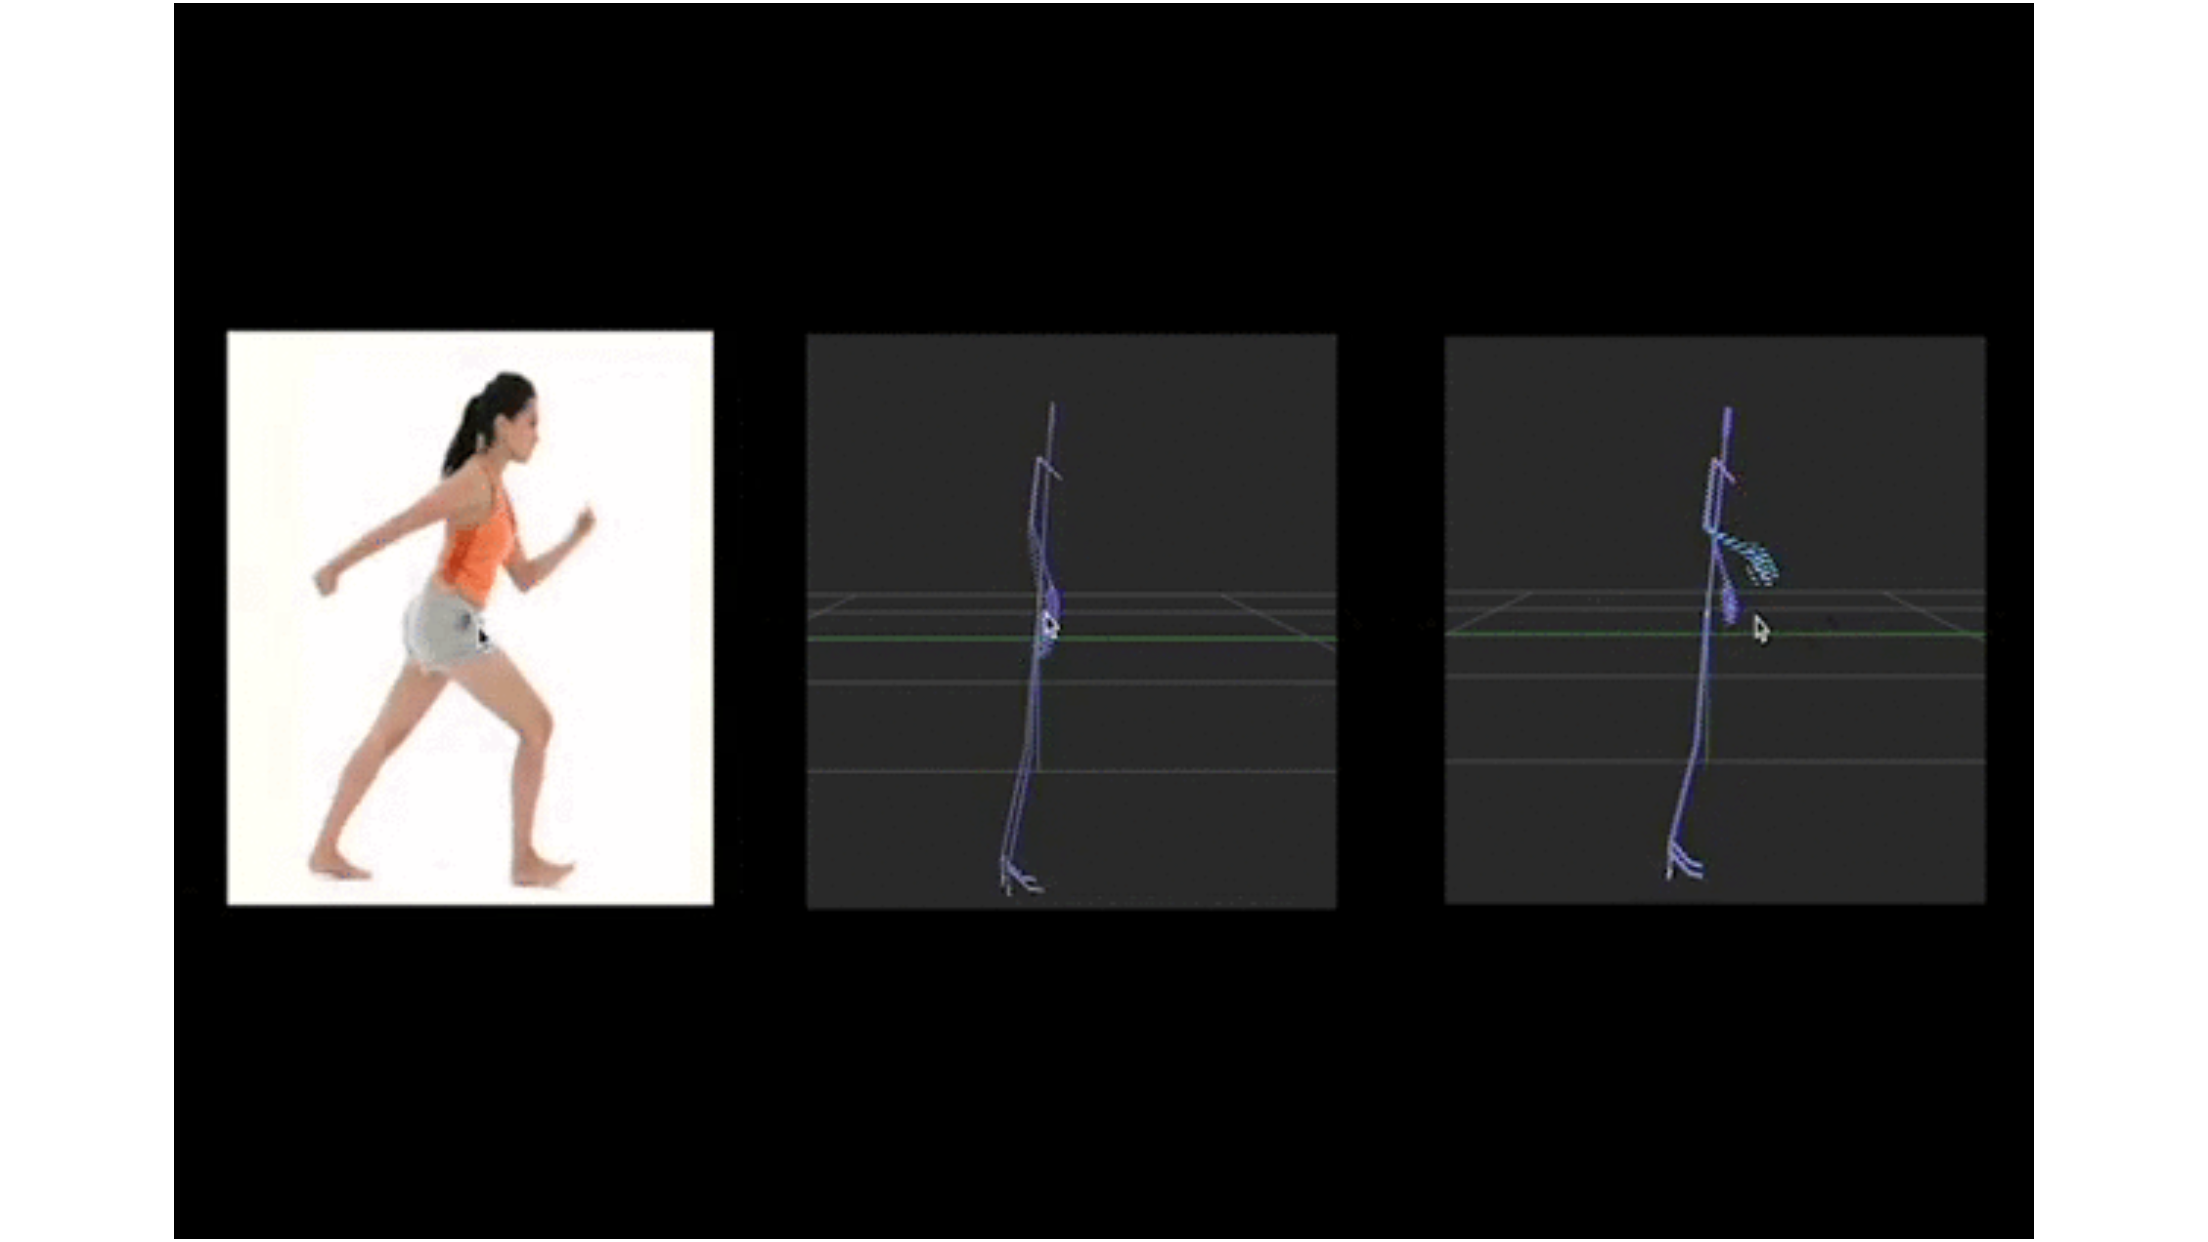
\includegraphics[width=0.3\textwidth]{2dtobvh1}
}
\subfigure[] {
\label{fig:2dtobvh2}
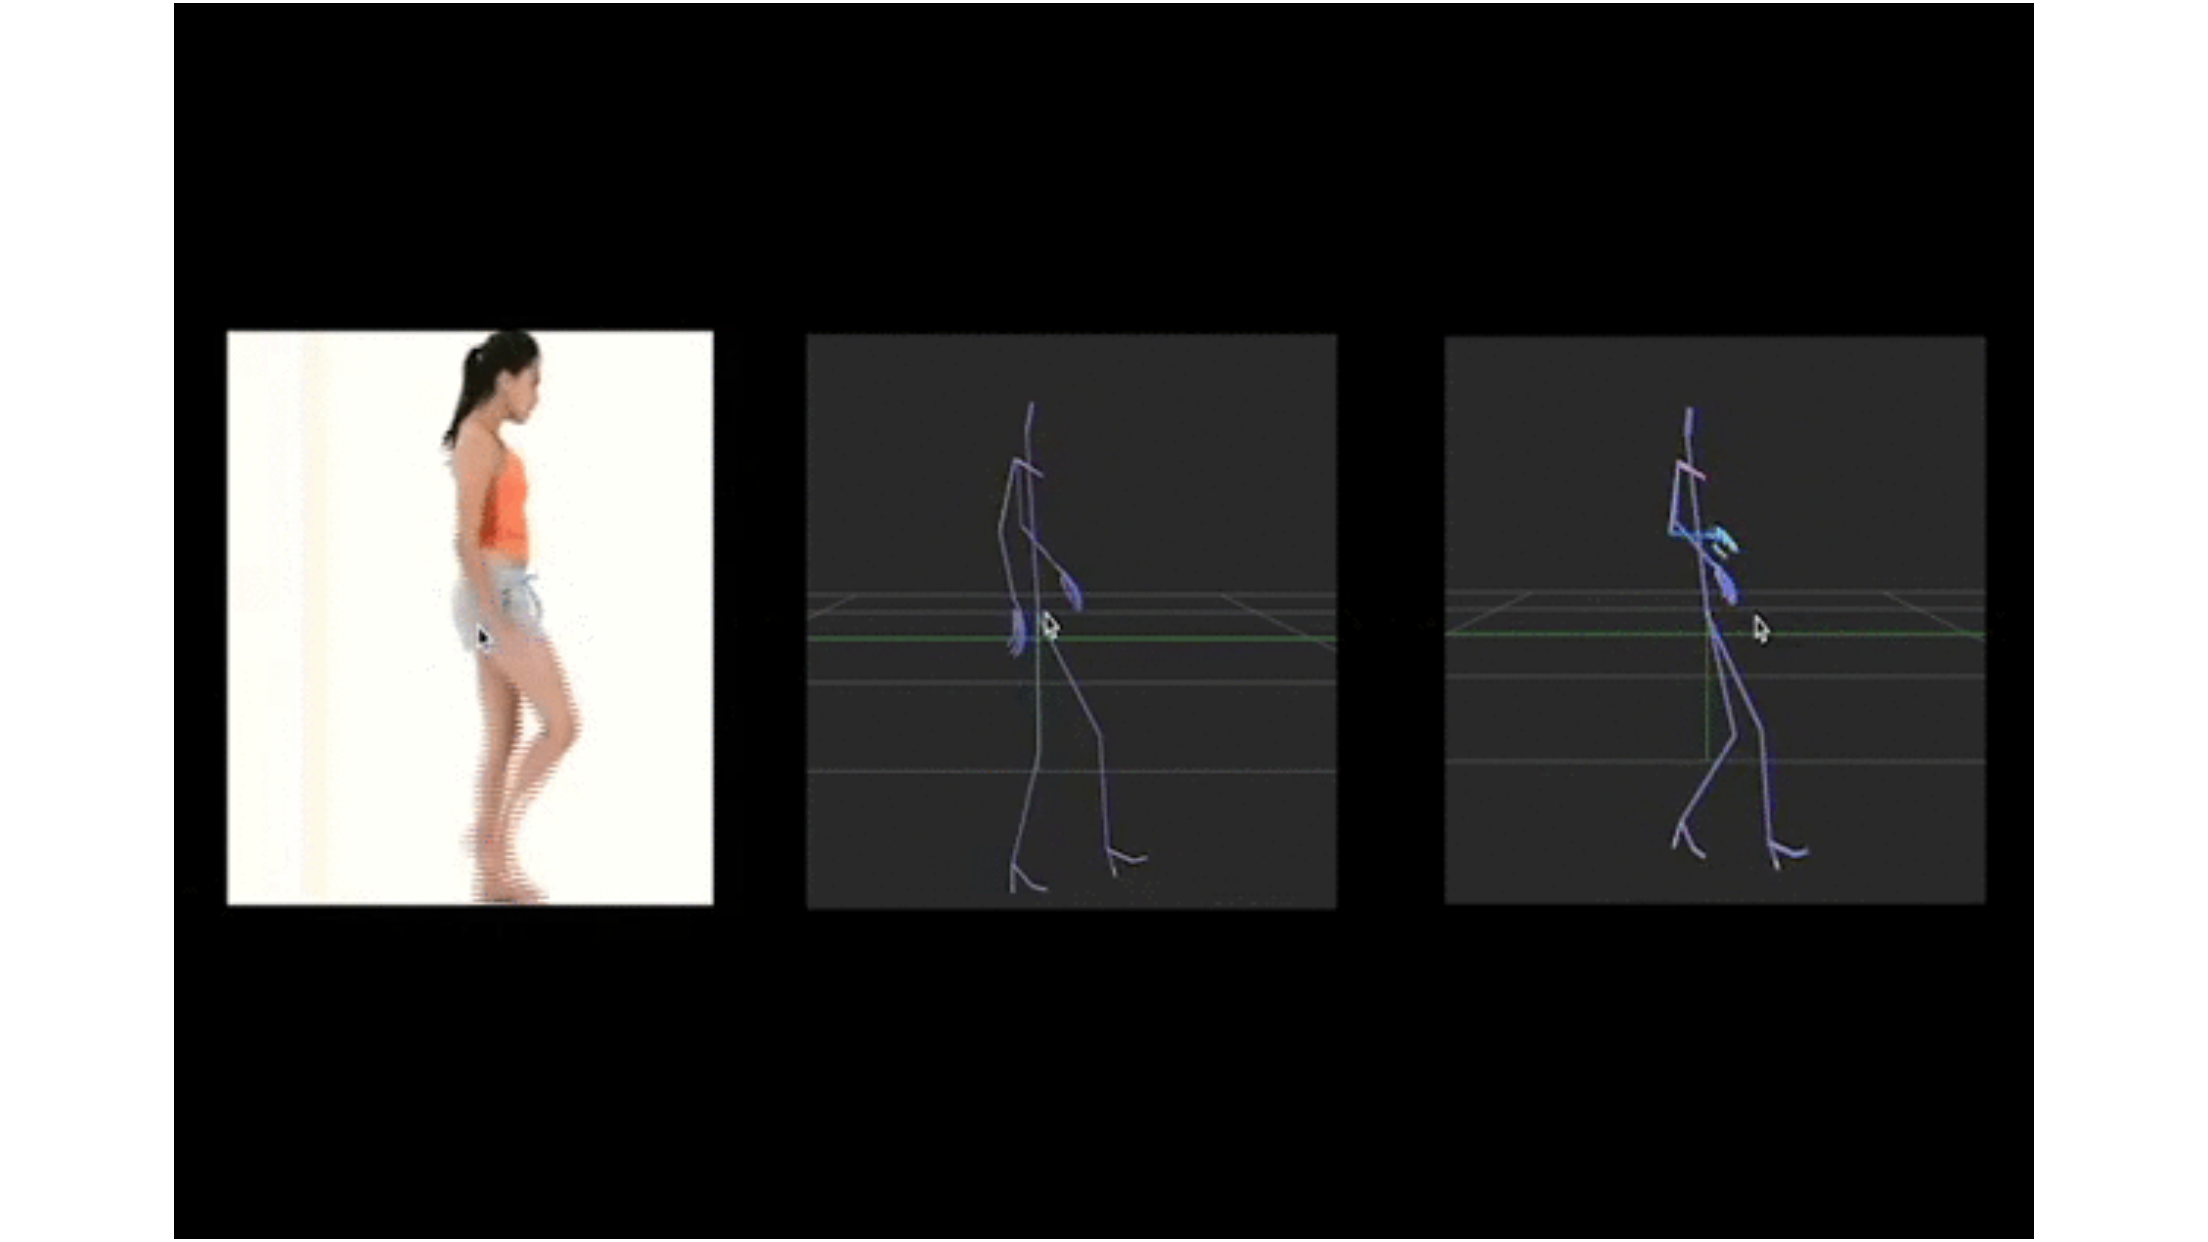
\includegraphics[width=0.3\textwidth]{2dtobvh2}
}
\subfigure[] {
\label{fig:2dtobvh3}
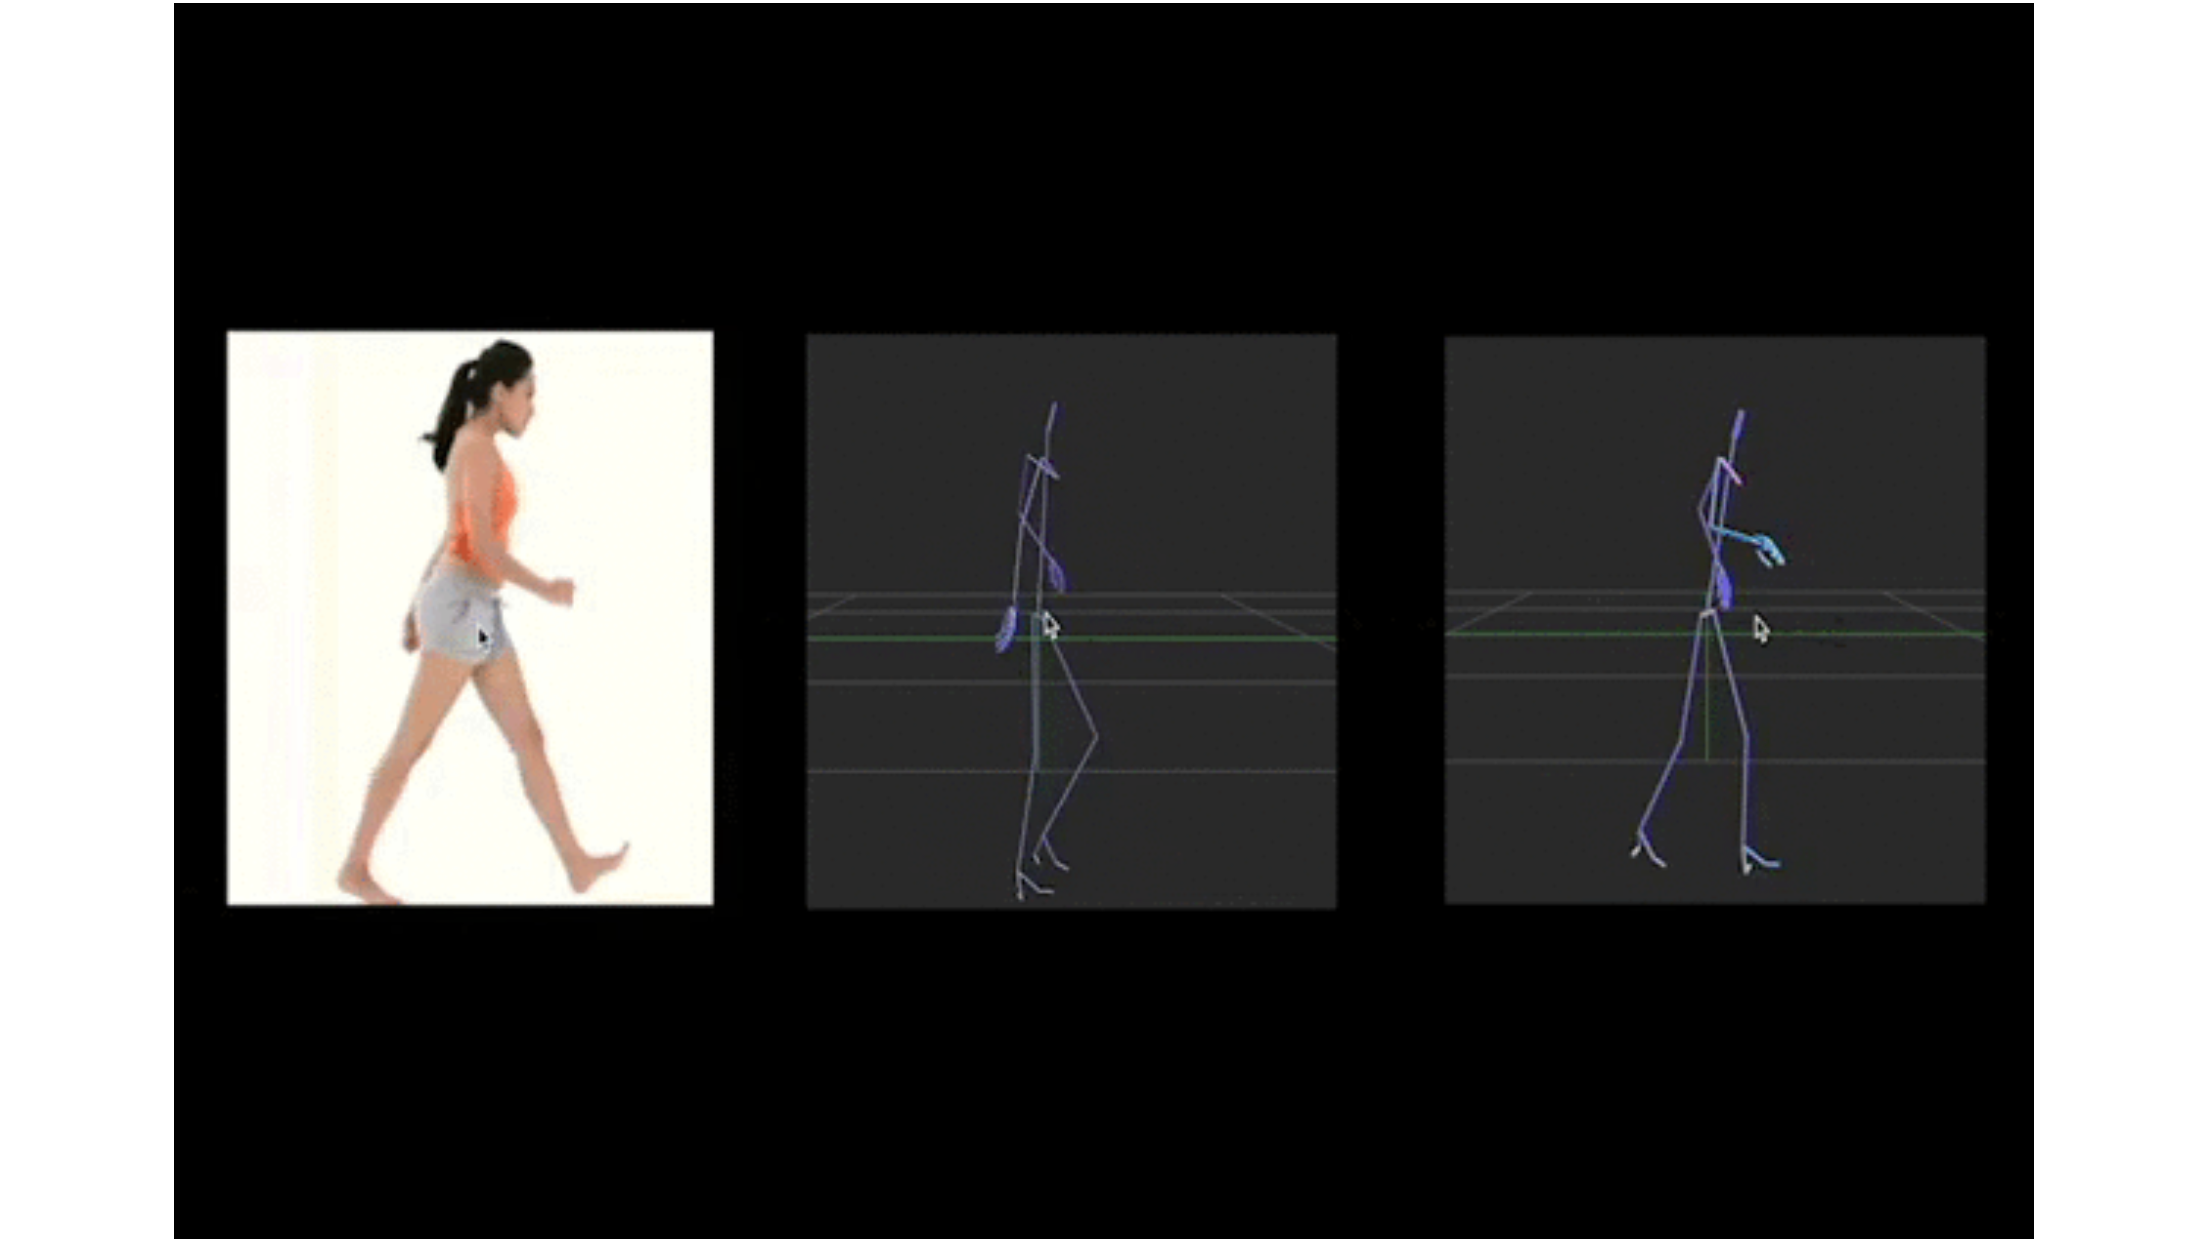
\includegraphics[width=0.3\textwidth]{2dtobvh3}
}
\caption{2D图像到BVH文件转换}
\label{fig:2dtobvh}
\end{figure}
如\cref{fig:2dtobvh}静态所示(左边为原始图片,中间为原始的姿态估计的结果\cite{kanazawa2018end},右边为运用$\mathbf{IK}$解算器修正后的图片),原始的姿态估计结果,有一些动作不符合人体骨骼活动的自然规律,例如肘关节向外翻转。但与此同时可以注意到,某一些关节,例如肩关节和腕关节,在姿态估计中的准确度远远高于肘关节这类活动范围更大的关节。所以将$\mathbf{IK}$解算器姿态估计问题中时,以右手臂为例,只考虑肩关节和腕关节的三维坐标,运用解算器反向推倒出肘关节的旋转角,然后再将其转换为世界坐标。在动态的GIF图中可以观察到,运用$\mathbf{IK}$解算器后的右手臂的弯曲更为自然。

除此之外,本文的去噪滤波器在姿态估计中也不可忽视。\cref{fig:2dtobvh}中的姿态已经经过去噪滤波器降噪处理过。在动态的GIF中,原始的姿态估计结果的抖动非常明显,甚至root关节点的世界坐标都呈现出不规律的抖动;但在运用了本文的去噪滤波器方法后,整体的运动消除了抖动,呈现出平滑效果,符合人体运动规律。


\section{讨论}{Discussion}

\subsection{不同网络结构的比较}{Comparison of Different Network Structures}
图\ref{fig:comparison_structure}验证了本文的网络选择的有效性,将其与其他流行网络进行性能比较,包括卷积神经网络(CNN),全连接神经网络(FCN)和生成性对抗网络(GAN)。这些网络的实现代码和模型在公开Github上(请参阅本文~\ref{sec:implementation}中的链接)

结果表明,具有相当小节点的RNN实现了与比其节点多的FCN相当的性能。因为RNN具有对时序序列表现更加优秀的特性,而本文中提出的对原始的数据经过额外的整合,加入了时间关联性,使之更符合RNN网络输入数据的特征要求。同时,FCN比起RNN非常可能导致过拟合问题,虽然在训练集上表现相当,但在测试集上FCN的表现远远不如RNN。在实际情况中,FCN只学习训练集的数据,相当于记忆了一个庞大的数据库,测试集上的损失函数并未明显下降,从另一方面证明FCN网络并未学习到如何求解$\mathbf{IK}$问题。

实验结果同样证明,CNN和GAN在本文的案例中不能产生令人满意的表现。CNN在实验过程,损失函数始终无法下降;GAN的调节参数过于复杂,且该问题是一个典型的监督学习问题,GAN的学习特征与之并不符合,所以GAN网络的损失函数一直无法收敛也可以得到解释。
\begin{figure}[!htbp]
	\centering
	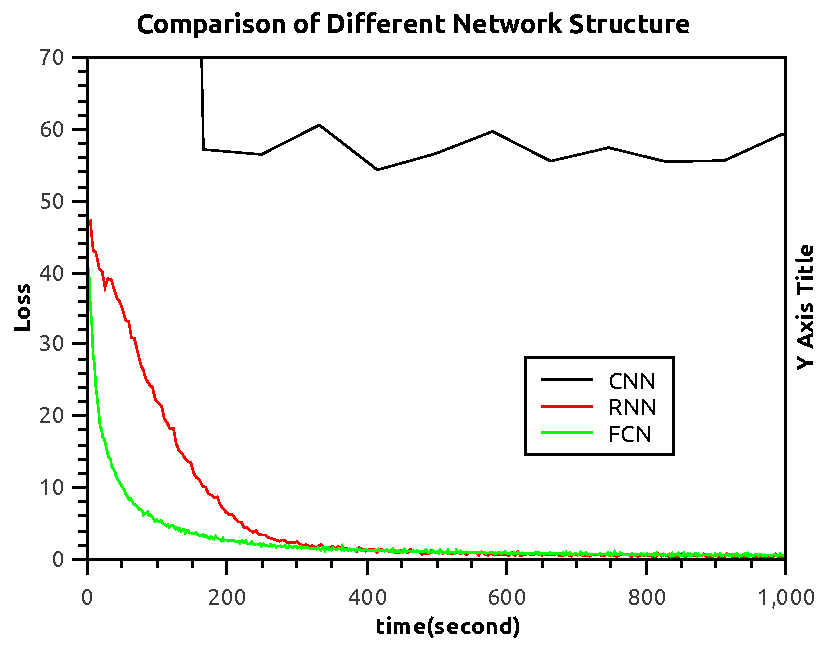
\includegraphics[width=0.75\linewidth]{comparison_structure.pdf}
	\caption[]{\label{fig:comparison_structure}
		不同网络模式的学习性能比较
	}
\end{figure}
\subsection{不同帧数输入的比较}{Comparison of Different Number of Input Frames}
\label{sec:different_nums}
\begin{figure}[!htbp]
	\centering
	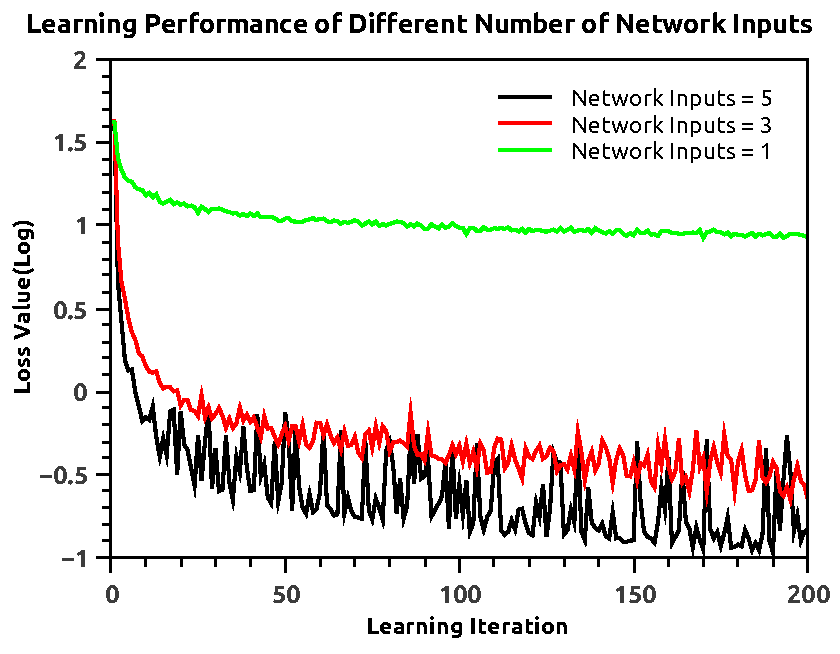
\includegraphics[width=0.75\linewidth]{comparison_num_inputs.pdf}
	\caption[]{\label{fig:comparison_num_inputs}
		不同输入帧数输入的网络学习性能比较
	}
\end{figure}
图\ref{fig:comparison_num_inputs}比较了当不同数量的帧用作网络输入时的学习性能。 该图表明,当单个帧用作网络输入时,学习性能不会产生令人满意的结果。实验中,将输入一帧的训练后的模型经过反算得到的BVH文件播放后,呈现出了巨大的抖动,且不符合人体运动规律。当增加帧数作为输入时,学习性能得到改善,但损失的方差同时也稍微更大。实验中,如\cref{fig:comparison_num_inputs2}所示,试验了输入7帧以上的结果,并没有太大的提升效果。为了学习性能、内存空间和稳定性的平衡,本文选取网络输入为5。
\begin{figure}[!htbp]
	\centering
	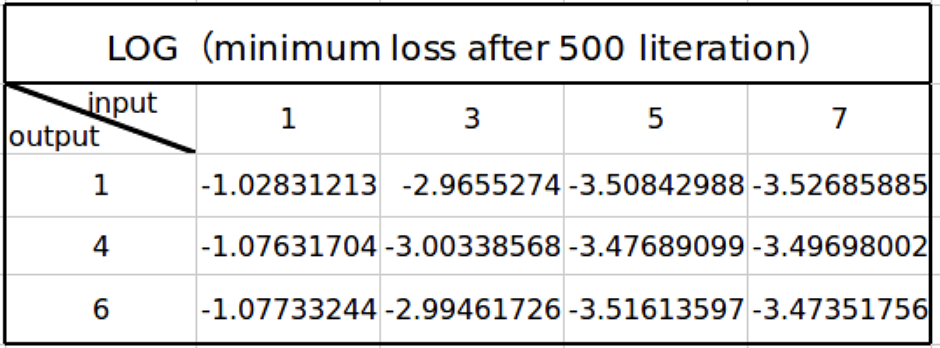
\includegraphics[width=0.75\linewidth]{comparison_num_inputs_2}
	\caption[]{\label{fig:comparison_num_inputs2}
		不同输入帧数和输出帧数的网络学习性能比较
	}
\end{figure}
\subsection{左臂和右臂的比较}{Comparison of Left and Right Arms}
图\ref{fig:comparison_left_right}比较了求解左侧手臂和右侧手臂时IK求解器的学习性能。
两种情况下的网络学习表现相似,只是左臂的函数损失相对较小且更稳定(因为损失函数做了$log$变换,将原来的细节进行了放大,实际情况中,二者差别更小一些)。这种差异应该是由于右臂负责更复杂的运动造成的(除了以左手为惯用手的少数群体)。在CMU的Mocap数据库中,经过排查后,几乎没有左撇子的参与者(考察了篮球运动类似的需要区分左右手的情况)。与左臂相比,一个以右手为惯用手的人右臂往往负责具有更高的复杂性的动作,活动范围也更大。这是导致右臂的$\mathbf{IK}$的IK解算器具有更高的函数损失和更多的抖动变化的主要原因。
\begin{figure}[!htbp]
	\centering
	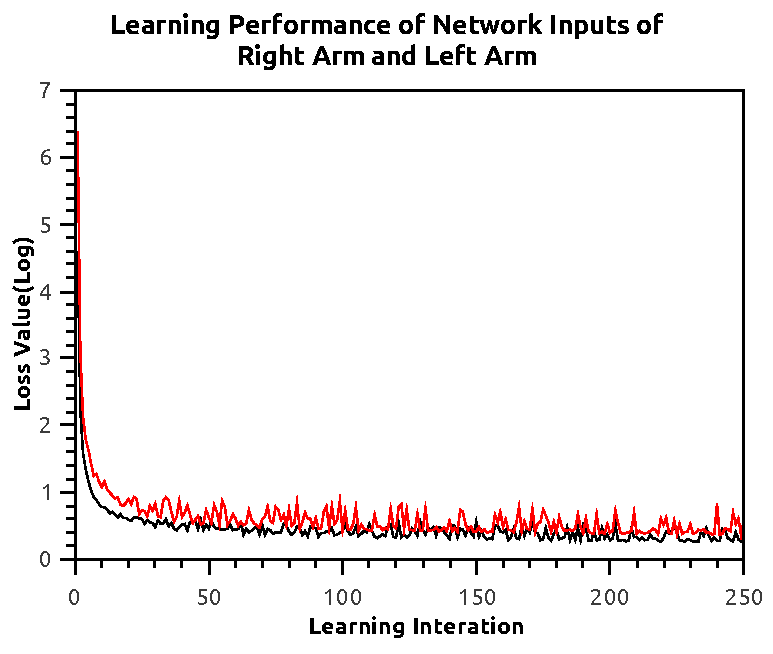
\includegraphics[width=0.75\linewidth]{comparison_left_right.pdf}
	\caption[]{\label{fig:comparison_left_right}
		左臂和右臂的网络学习性能表现
	}
\end{figure}
\subsection{手臂和腿的比较}{Comparison of Arm and Foot}
图\ref{fig:comparison_foot_arm}比较了在求解右侧的腿部和手臂的IK问题时网络的学习性能。结果表明,脚的解算器的平均损失和方差远小于手臂的平均损失和方差。这反映了一个事实,手部运动比脚部运动更加细腻和复杂。根据人类常识,手进行的活动比腿部更为复杂,且数量更多,且由于韧带和人体结构的影响,手臂的活动范围远远大于腿部。
\begin{figure}[!htbp]
	\centering
	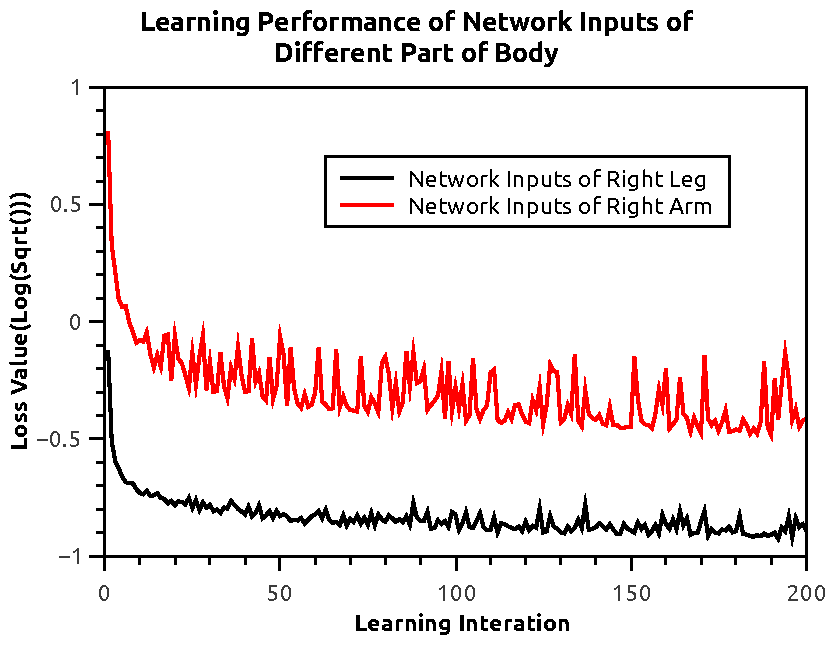
\includegraphics[width=0.75\linewidth]{comparison_foot_arm}
	\caption[]{\label{fig:comparison_foot_arm}
		手臂和腿部的网络学习性能比较
	}
\end{figure}
\subsection{重定位动作至不同肢体长度角色}{Motion Retargetting to Characters with Different Limb Lengths}
\label{sec:Retargetting}
由于末端执行器的位置用肢长度进行了标准化,以右手臂为例,
\begin{displaymath}
\overrightarrow{AC}=\frac{(\overrightarrow{AB}+\overrightarrow{BC})}{(\left|\overrightarrow{AB}\right|+\left|\overrightarrow{BC}\right|)}
\end{displaymath}
式中$\overrightarrow{AB}$、$\overrightarrow{BC}$、$\overrightarrow{AC}$皆为三维向量,分别表示右大臂、右小臂和IK解算器输入的向量.$\mathbf{A}$表示肩关节的位置,$\mathbf{B}$表示肘关节位置,$\mathbf{C}$表示腕关节位置.\cref{fig:limb_length}展示了本文方法可以推广到具有不同肢长的角色的IK问题的求解.三张图内虽然肢体长度差别巨大,但在BVH PLAYER中进行播放时,手臂和腿部的活动并未出现滑动和抖动,皆符合人体运动的规律。
\begin{figure}
\centering
\subfigure[站立动作(正常肢体长度)] {
\label{fig:standard}
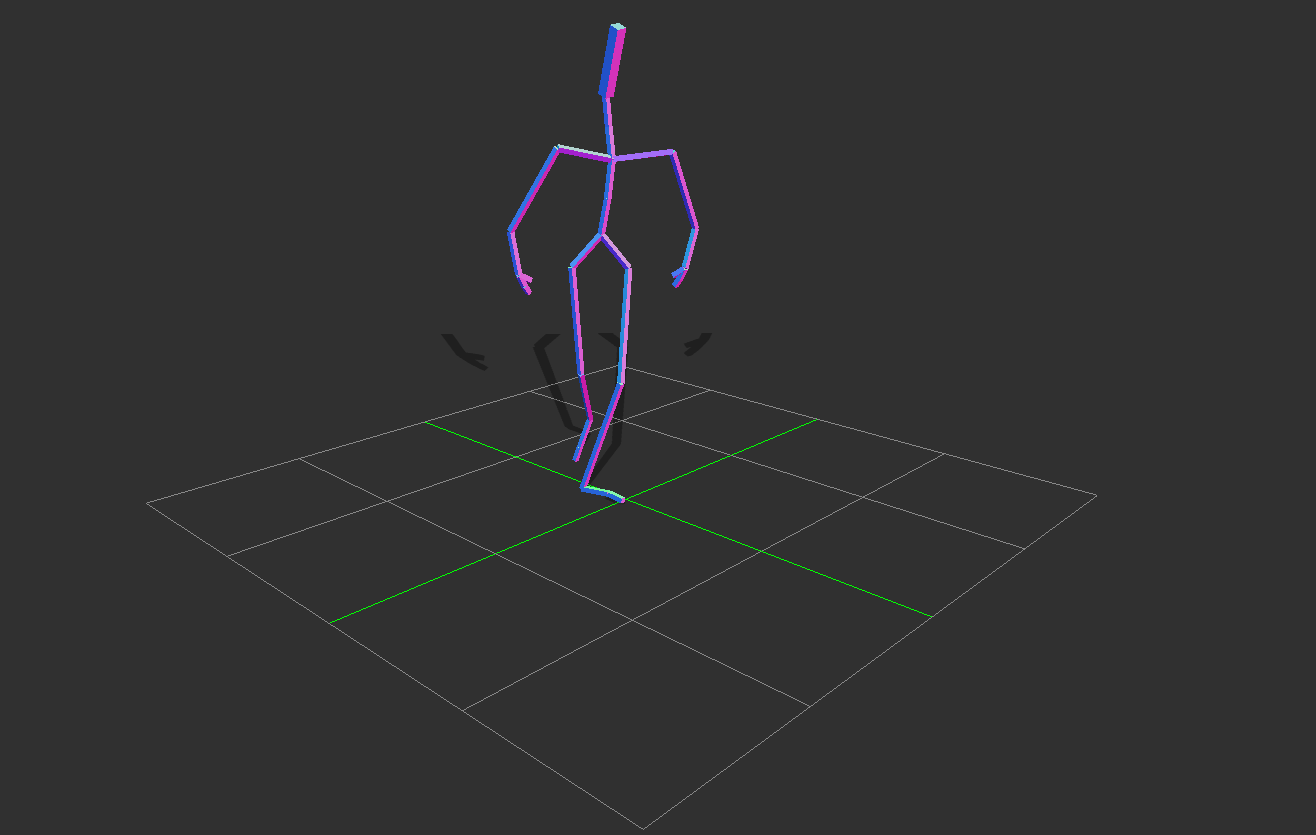
\includegraphics[width=0.3\textwidth]{standard}
}
\subfigure[站立动作(短臂)] {
\label{fig:short_arm}
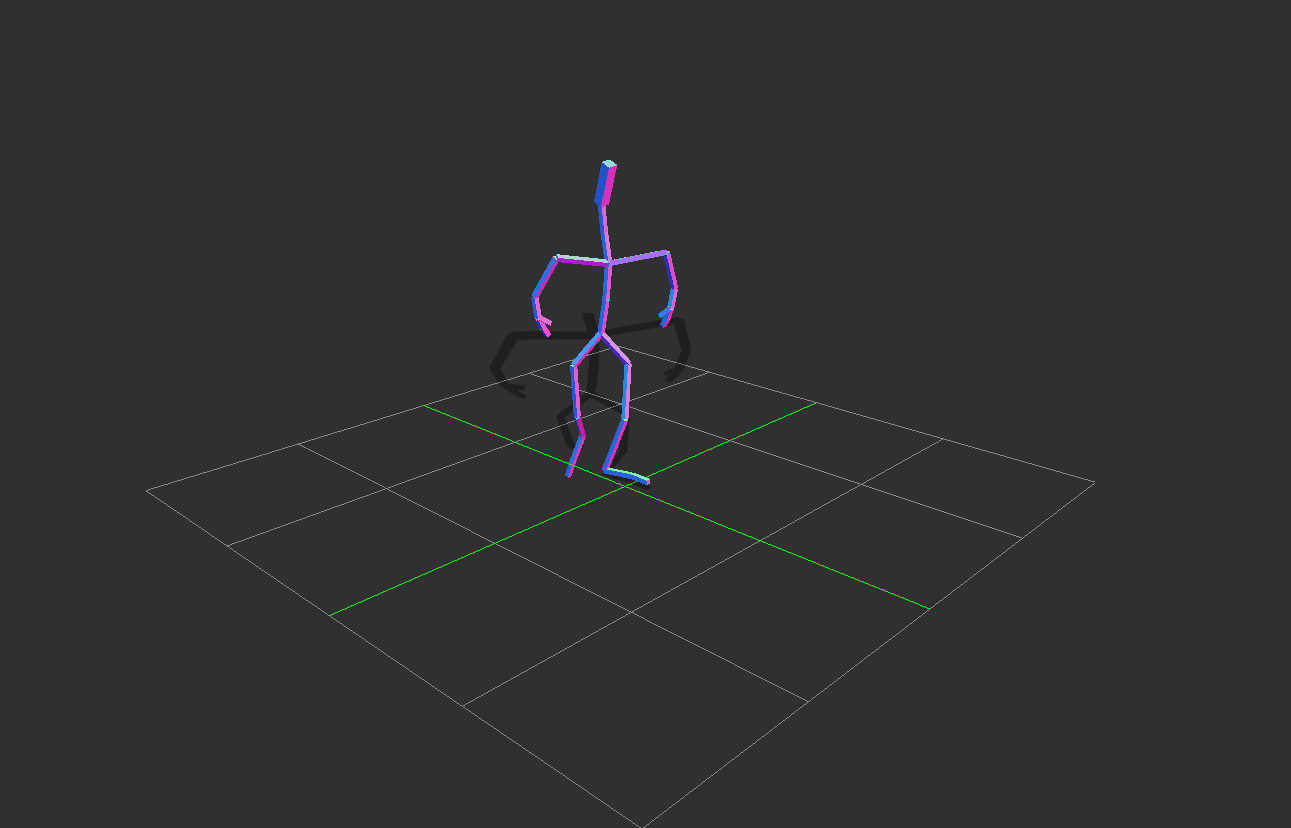
\includegraphics[width=0.3\textwidth]{short_arm}
}
\subfigure[站立动作(短腿)] {
\label{fig:short_leg}
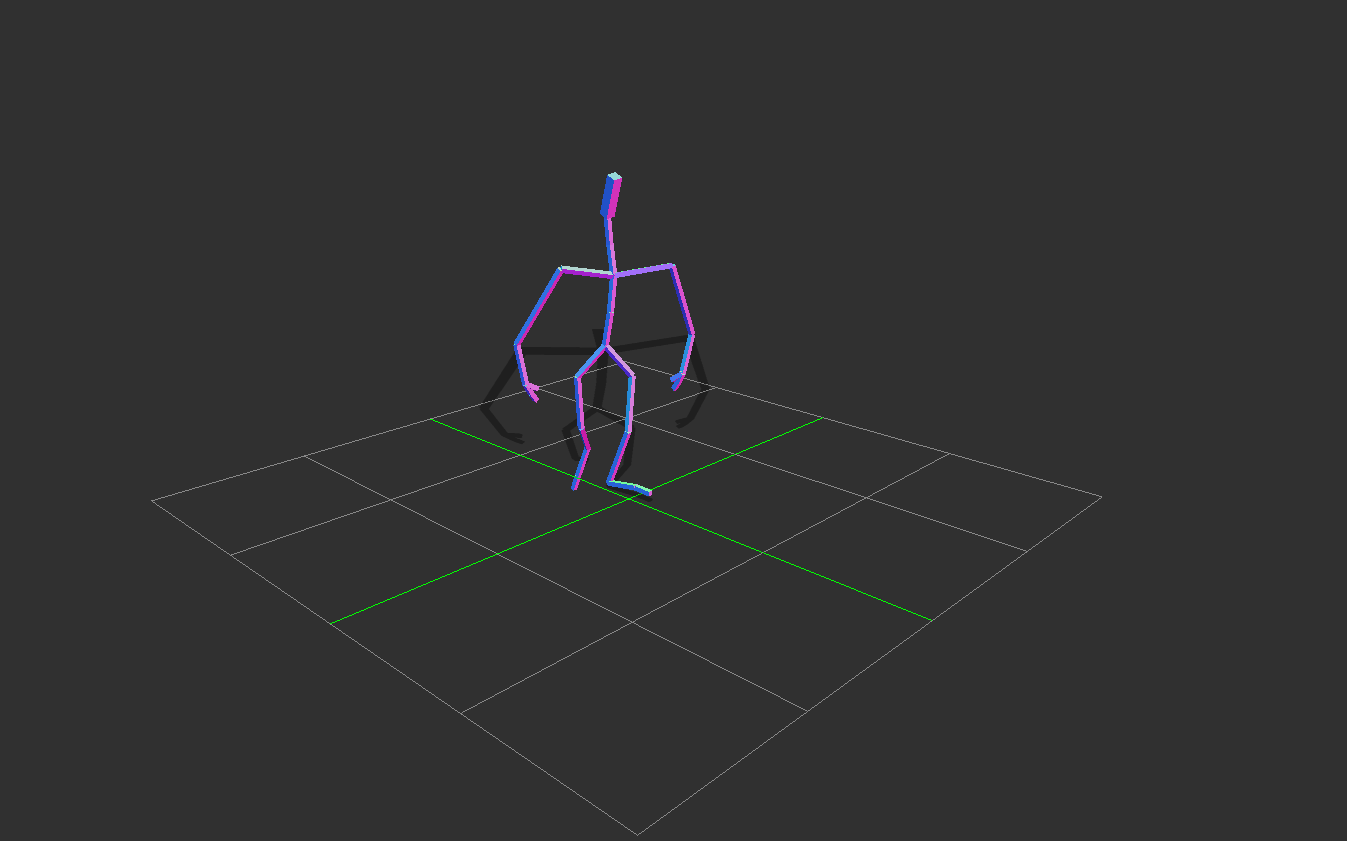
\includegraphics[width=0.3\textwidth]{short_leg}
}
\caption{不同肢体长度角色的合成动作}
\label{fig:limb_length}
\end{figure}
\section{应用}{Application}
\subsection{关键帧轨迹}{Trajectory Key-framing}
本文涉及工作的一个直接应用就是关键帧轨迹。用户将末端效应器的运动轨迹拟合为一条样条曲线,IK解算器可以自动生成沿着身体关节连接方向的各个关节角度,以获得四肢完整的关节运动轨迹。该任务首先应使用均匀参数对样条曲线进行采样,其次还需要将连续多帧合并为一段输入作为神经网络的输入。
\subsection{实时动作压缩}{Real-time Motion Compression}
本文方法的另一个应用是动作压缩。 在标准类型的动作文件(例如BVH格式)中,角色动作用根关节的全局变换和子关节相对于父关节的偏移和方向来描述。 鉴于IK求解器具有高精度,因此用末端执行器的位置替换关节的角度和方向是足够的。 这种方法可以将动作的存储空间减少至少$50\%$,这对于实时应用程序中的数据传输非常的重要。

\subsection{频繁交互环境中的运动合成}{Motion Synthesis in Contact-rich Environment}
\cref{fig:train_screenshot}和\cref{fig:test_screenshot}均展示了在涉及频繁的肢体与环境接触的情景,本文所述的方法仍具有合成自然的动作的能力。
